\begin{theo}[Convexity for $C^1$ functions]{ConvexityC1}
    \begin{minipage}{0.60\textwidth}
        Assume that $f: \ \Omega \rightarrow \R$ is continuously differentiable and $\Omega$ is convex. Then holds that $f$ is convex if and only if 
        \begin{equation*}
            \forall x,y \in \Omega: \ f(y) \geq f(x) + \nabla f(x)^T(y-x)
        \end{equation*}
        i\@.e\@. tangents lie below the graph.
    \end{minipage}
    \begin{minipage}{0.3\textwidth}
        \begin{center}
            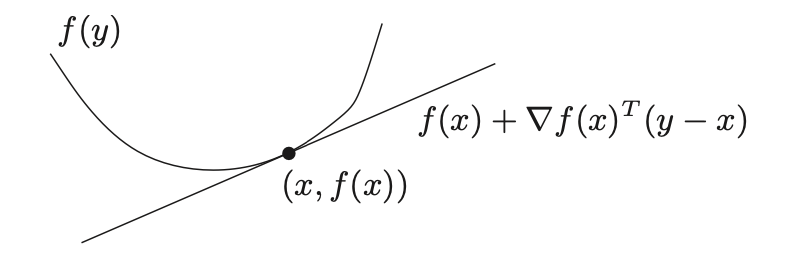
\includegraphics[scale = 0.45]{Images/Fundamental/C1Convexity.png}
        \end{center}
    \end{minipage}
\end{theo}

\begin{prf}[Convexity for $C^1$ functions]{prfConvexityC1}
    ``$\Rightarrow$'': Due to convexity of $f$ holds for given $x,y \in \Omega$  and for any $\lambda \in [0,1]$ that
    \begin{equation*}
        f(x + \lambda(y-x)) - f(x) \leq \lambda(f(y) - f(x)).
    \end{equation*}
    and therefore that 
    \begin{equation*}
        \nabla f(x)^T(y-x) 
            = \lim_{\lambda \rightarrow 0}  \frac{f(x + \lambda(y-x)) - f(x)}{\lambda}
            \leq \frac{f(y) - f(x)}{y-x}.
    \end{equation*}

    ``$\Leftarrow$'': To prove that $z = x + \lambda(y-x) = (1-\lambda)x + \lambda y$ holds that $f(z) \leq (1-\lambda)f(x) + \lambda f(y)$, we can use the equation from Theorem~\ref*{ConvexityC1} twice to get
    \begin{equation*}
        f(x) \geq f(z) + \nabla f(z)^T(x-z) \ \ \text{and} \ \ f(y) \geq f(z) + \nabla f(z)^T(y-z),
    \end{equation*}
    which yield, when weighted with $(1-\lambda)$ and $\lambda$ respectively, that
    \begin{equation*}
        (1-\lambda)f(x) + \lambda f(y) \geq f(z) + \nabla f(z)^T \underset{= 0}{\underbrace{\left[(1-\lambda)(x-z) + \lambda(y-z)\right]}}
    \end{equation*}
    \vspace{-0.75cm}
\end{prf}

